\begin{refsection} 
 
\chapter{Automation} \label{chapter:automation}
 
\setlength{\epigraphwidth}{3in} 
\epigraph{\textit{``Give me six hours to chop down a tree and I will spend the 
first four sharpening the axe.''}}{Abraham Lincoln} 
\vspace{3em} 
 
Once the budding computational scientist has learned the basics on how to use 
their \textit{ab initio} code of choice, he or she will begin their career by 
manually setting up the required input files, usually from a set copied from a 
previous calculation. This approach, however, has several downsides. Manually 
adjusting the input tags for each calculation is very time consuming, 
especially when a lot of calculations have to be performed. Certainly, any 
supervisor can agree this time would be better spent analysing results and 
writing papers. Moreover, some properties cannot be feasibly calculated in 
such a manner, as the time required to set up all of the calculations would be 
prohibitively large. Finally, adjusting input settings manually often leads to 
user-related errors, especially when calculations are set up late at night.  

When a large amount of similar calculations have to be performed, it is much 
more sensible to design an automated workflow that performs the required steps 
for whatever series of calculations you have in mind. Although it is certainly 
possible to write your own scripts, there are already several software 
packages available that provide a useful framework for this purpose, based on 
for example \href{http://pymatgen.org/}{pymatgen}~\cite{Ong2013} or the 
\href{https://wiki.fysik.dtu.dk/ase/}{Atomic Simulation Environment} 
(ASE)~\cite{Larsen2017}. For my work, I have exclusively relied on 
\href{https://materialsproject.github.io/fireworks/index.html}{Fireworks}~\cite{Jain2015}, 
a powerful Python package for designing, executing and managing computational 
workflows. 
 
In this chapter I give an overview of all of the workflows that were used to 
calculate the various properties required for my research. I also explain some 
more technical details of performing certain calculations using our chosen 
implementation of the DFT formalism: the \href{https://www.vasp.at/}{Vienna ab 
initio simulation package} (VASP). After the short introduction in 
Section~\ref{automation:sec-intro}, the chapter continues with detailing the 
building blocks of a workflow in Section~\ref{automation:sec-firetasks}. Next, 
Section~\ref{automation:sec-workflows} describes the workflows used to obtain 
the results presented in future chapters. For each workflow, there is a 
corresponding example Jupyter notebook that details and executes the various 
steps performed to set up the calculation and run the workflow. Finally, 
Section~\ref{automation:sec-computational} discusses some details on how to  
adjust the computational settings used for the workflows. 
 
\pagebreak 
 
\section{Introduction} \label{automation:sec-intro} 
 
Many \textit{ab initio} methods for calculating properties rely on a fairly 
fixed algorithm of reoccurring steps. Even when the exact steps depend on the 
result of a previous calculation, it is usually feasible to come up with some 
sort of well-defined schematic, or workflow, on how to best calculate the 
desired property for any structure. Fireworks is a well-established Python 
package for designing such a workflow. 
 
As an example, say you want to calculate the density of states of a certain 
structure, e.g. the chalcopyrite phase of \ce{CuInSe2}. After obtaining an 
initial geometry, either by constructing it manually, or - more conveniently - 
by extracting it from a trustworthy database~\cite{Jain2013}, the first step 
is to optimize the structure computationally. Once you have obtained the 
optimized geometry, the next step is calculate the density of states using two 
consecutive VASP calculations: first one to calculate the charge 
density of the electrons using a relatively sparse k-point sampling of the 
Brillouin zone, then a calculation that keeps the charge density fixed and 
determines the energies of the electronic states with a much denser k-point 
mesh. Such a fixed process for calculating a specific property is an ideal 
application of a workflow, especially if you want to obtain this property for 
a large number of structures.  
 
Workflows are assembled from connected steps, called 
\href{https://github.com/materialsproject/fireworks/blob/master/fireworks/core/firework.py#L196}{\code{Firework}}s, 
which in turn consist of a set of consecutive 
\href{https://github.com/materialsproject/fireworks/blob/master/fireworks/core/firework.py#L46}{\code{Firetask}}s. 
How the various tasks that need to be performed are organized in 
\code{Firework}s and \code{Firetask}s is up to the user, but the developers do 
provide some 
\href{https://materialsproject.github.io/fireworks/design_tips.html}{general 
guidelines} on how to design your workflows. All of my workflows were 
constructed by bundling all of the tasks required for a single VASP 
calculation into one \code{Firework}, and then connecting these 
\code{Firework}s to create a workflow for each of the properties required for 
my research. 
 
\section{Firetasks} \label{automation:sec-firetasks} 
 
Let's begin with an overview of the smallest building blocks of the workflows: 
the \code{Firetask}. Each \code{Firework} of the workflow consists of a list 
of \code{Firetask}s, which are executed sequentially in the order specified by 
the user when initializing the \code{Firework}. While the workflow is 
running, all \code{Firetask}s have access to the \textit{spec} of their parent 
\code{Firework} (\code{\_fw\_spec}). This allows the user 
to easily pass information between tasks. The spec also contains the launch 
directory of the \code{Firework}, so the initial \code{Firetask} is executed 
in this directory. 
 
\subsection{\texttt{WriteVaspFromIOSet}} 
\label{automation:sec-WriteVaspFromIOSet} 
 
As the name implies, the \code{WriteVaspFromIOSet} task writes the 
VASP input files into the current directory. Each calculation is 
defined by an input set, i.e. a class derived from \code{pymatgen}'s 
\code{DictSet} class. This class does a few things: 
 
\begin{itemize} 
 
\item Load the basic configuration from a YAML\footnote{YAML Ain't Markup 
Language; IT people love recursion, also in their acronyms.} file. This file 
contains the settings for each of the VASP input files (See 
Appendix~\ref{appendix:sec-VASP}). Here's an (truncated) example: 
\begin{verbatim} 
INCAR: 
  ALGO: Fast 
  EDIFF: 1.0e-06 
  ENCUT: 500 
  ISMEAR: -5 
  ... 
KPOINTS: 
  grid_density: 3000 
POTCAR: 
  Ac: Ac 
  Ag: Ag 
  Al: Al 
  Am: Am 
  Ar: Ar 
  As: As 
  At: At_d 
  ... 
\end{verbatim} 
Besides the \vasp{INCAR} tags, the YAML file also specifies the 
\link{dft:sec-kpoints}{sampling of the Brillouin zone}. This is done based on 
a specified density, as the number of k-points should of course depend on the 
size of the reciprocal unit cell. Finally, the \vasp{POTCAR} file is specified 
for each element, which mainly determines the number of valence (and core) 
electrons to consider in the \link{dft:sec-PAW}{PAW formalism}. Each 
\vasp{POTCAR} file has a specific name, e.g. default file for \ce{At} only 
considers the 6$p$ electrons as valence electrons, but the \texttt{At\_d} file 
also includes the 5$d$ electrons. 
 
\item Make adjustments to the configuration based on the structure and what 
calculation has to be performed. For example, in case the provided structure 
has magnetic moments specified, the \vasp{ISPIN} tag is set to 2 in order to 
perform a spin polarized calculation. Or, for a geometry optimization of a 
\link{automation:sec-surface}{slab}, selective dynamics is applied to fix a 
certain selection of the atoms based on user-provided settings. Based on the 
input set, the configuration of the YAML file is also adjusted, e.g. 
\code{SlabOptimizeSet} is based on the \texttt{optimizeSet.yaml} file, but 
automatically sets \vasp{ISIF} to 2, fixing the unit cell of the calculation. 
 
\item Write the output files using the \code{write\_input()} method. Every 
\code{DictSet} subclass requires the structure as an input argument, so based 
on the structure and configuration, all of the VASP input files can 
be written. Note that the \vasp{MAGMOM} tag, which specifies the magnetic 
moments in the structure, is also automatically added to the \vasp{INCAR} 
file, which can be a real headache to do manually for large complicated 
structures. 
 
\end{itemize} 
 
The default method for initializing the \code{WriteVaspFromIOSet} class is by 
providing either an initialized input set or the structure and the name of the 
input set of the calculation. However, in some cases the structure cannot be 
provided when the workflow is set up, as it relies on a previous geometry 
optimization. In this case the structure will be extracted from the directory 
of the parent \code{Firework}. Note that if the input set is defined by the 
name, either a structure or parent \code{Firework} must be provided, else the 
\code{Firetask} has no recourse for obtaining the structure. 
 
\subsection{\texttt{VaspParallelizationTask}} 
\label{automation:sec-VaspParallelizationTask} 
 
As most DFT calculations require a substantial amount of computational 
resources, it is important to properly parallelize the workload over the 
various nodes/cores of a cluster, as failing to do so can severely affect the 
performance. For VASP, the parallelization can be controlled by 
several parameters: 
 
\begin{itemize} 

\item \href{https://cms.mpi.univie.ac.at/wiki/index.php/KPAR}{\texttt{KPAR}}: 
Determines the parallelization over the k-points. VASP treats 
\texttt{KPAR} k-points in parallel, i.e. it divides the number of available cores (\texttt{\#CORES}) and 
k-points in \texttt{KPAR} groups and then assigns each group of cores to work 
on a group of k-points, one k-point at a time. As \texttt{KPAR} divides the 
k-points of the calculation in groups, \texttt{KPAR} is optimally chosen to be 
a divisor of the number of k-points. However, this rule should \textbf{not} be 
set in stone, as often choosing a higher \texttt{KPAR} that is not a divisor 
of the number of nodes can result in an improved optimization. 
 
\item \href{https://cms.mpi.univie.ac.at/wiki/index.php/NPAR}{\texttt{NPAR}}: 
A second way in which VASP allows parallelization is over the 
electronic bands. For each k-point, there are \verb|#CORES|/\verb|KPAR| cores 
working on it at a single time. Using \verb|NPAR|, we can further divide the 
cores per k-point into \verb|NPAR| groups, i.e. treat \verb|NPAR| bands in 
parallel using \verb|#CORES|/\verb|KPAR|/\verb|NPAR| cores. Note that similar 
to the \verb|KPAR| and the number of k-points,  \verb|NPAR| should optimally 
be a divisor of the number of bands to avoid inactive cores. VASP 
actually enforces this by setting the number of bands (\vasp{NBANDS}) to the 
smallest multiple of \verb|NPAR| higher than the requested (or default) bands. 
 
\item 
\href{https://cms.mpi.univie.ac.at/wiki/index.php/NCORE}{\texttt{NCORE}}: The 
number of cores that are working together on an individual band. For a 
specified \verb|NPAR|, \verb|NCORE| is automatically set using the following 
relation: 
\begin{equation*} 
\texttt{NCORE} = \frac{\texttt{\#CORES / \texttt{KPAR}}}{\texttt{NPAR}} 
\end{equation*} 
In other words, the user should specify either \verb|NPAR| or \verb|NCORE|, as 
they are directly connected. As is said in the VASP manual, 
\verb|NPAR| is preferred, i.e. if you do set both \verb|NPAR| and 
\verb|NCORE|, the \verb|NCORE| value is ignored. 
 
% \item \href{https://cms.mpi.univie.ac.at/wiki/index.php/LPLANE}{\texttt{LPLANE}}: \#TODO 
 
\item \href{https://cms.mpi.univie.ac.at/wiki/index.php/NSIM}{\texttt{NSIM}}: 
This input tag defines the number of bands that are treated simultaneously in 
the blocked mode of the \texttt{RMM-DIIS}\footnote{Residual minimisation/direct inversion in the iterative subspace~\cite{Wood1985}.} algorithm. This allows VASP 
to exploit matrix BLAS\footnote{Basic linear algebra subprograms.} operations instead of matrix-vector operations, which 
could lead to a speed up on some machines. Peter Larsson 
\href{https://www.nsc.liu.se/~pla/blog/2012/02/22/nparnsim/}{wrote an 
interesting blog post} on the topic. Overall, the gains are smaller compared to 
successfully utilizing \verb|NPAR| and \verb|KPAR|, but it might be worth 
experimenting with this value in case you rely on the \texttt{RMM-DIIS} 
algorithm. 
 
\end{itemize} 
 
As an example, consider the following parallelization settings for a 
calculation that uses 32 cores: \texttt{KPAR = 4}; \texttt{NPAR = 2}, shown 
schematically in Fig.~\ref{automation:fig-parallel}. First, the total number 
of cores is divided among \texttt{KPAR = 4} groups, resulting in 
\texttt{\#CORES/KPAR = 8} cores working on each group of kpoints. Next, the 
cores are split into \texttt{NPAR = 2} groups, which means that \texttt{NCORE 
= \#CORES/KPAR/NPAR} = 4 cores will be working simultaneously on each band. 
 
\begin{figure}[hb] 
\centering 
%%%%% Define Tikz colors and styles %%%%%

\definecolor{cores}{HTML}{173F5F}
\definecolor{kpar}{HTML}{3BAEA3}
\definecolor{npar}{HTML}{ED553B}

\tikzset{my lines/.style={
    black!30!white, line width = 0.2pt
}}

\tikzstyle{arrow} = [->, >=latex, very thick]
\tikzstyle{corebox} = [very thick, step=1, fill opacity=0.5]
\tikzstyle{connection} = [thick]

%%%%% TikZpicture %%%%%

\begin{tikzpicture}[scale=0.6, node distance=0.4em]

% Draw the core boxes
\draw [corebox, xshift=0.5cm, fill=cores] (7, 8) grid (15, 12) rectangle (7, 8);
\foreach \x in {0, 6, ..., 21}
    \draw [corebox, xshift=0.5cm, fill=kpar] (\x, 4) grid (\x +4, 6) rectangle (\x, 4);
\foreach \x in {0, 3, ..., 21}
    \draw [corebox, fill=npar] (\x, 0) grid (\x + 2,2) rectangle (\x, 0) ;

% Draw connections
\draw [connection] (11.5, 8) -- (11.5, 7);
\foreach \x in {2.5, 8.5, ..., 21}
    \draw [connection] (11.5, 7) -- (\x, 7) -- (\x, 6);
    
\foreach \x in {2.5, 8.5, ..., 21}{
    \draw [connection] (\x, 4) -- (\x, 3);
    \draw [connection] (\x, 3) -- (\x - 1.5, 3) -- (\x - 1.5, 2);
    \draw [connection] (\x, 3) -- (\x + 1.5, 3) -- (\x + 1.5, 2);
    }
    
% Annotation
\node [font=\Large, align=center] at (11.5, 12.5) {\texttt{\#CORES = 32}};
\draw [arrow] (-1, 9) -- node [rotate=90, above=0.3em] {\texttt{KPAR = 4}} (-1, 5.5);
\draw [arrow] (-1, 4.5) -- node [rotate=90, above=0.3em] {\texttt{NPAR = 2}} (-1, 1);

\end{tikzpicture} 
\caption{Schematic of a parallelization for 32 cores, \texttt{KPAR = 4}  and 
\texttt{NPAR = 2}.} 
\label{automation:fig-parallel} 
\end{figure} 
 
Most applications for calculation time on a higher Tier system, such as the 
\href{https://www.vscentrum.be/tier1}{BrEniac} cluster of the Flemish supercomputer center (VSC), or the 
\href{http://www.prace-ri.eu/}{PRACE} infrastructure of the European Union, 
require the user to demonstrate the scaling of their requested calculations is 
optimal. This involves testing a range of parallelization settings for an 
increasing number of nodes, and comparing the speed of the calculation at 
higher node usage in order to analyse the efficiency. An example of such an 
analysis can be found in Appendix~\ref{appendix:sec-parallel}. However, 
performing these tests for every structure/calculation in a workflow would 
defeat the purpose, as you would spend more time on running tests than 
actually producing results.  
 
\code{VaspParallelizationTask} is my humble approach to automating this 
process, based on a 
\href{https://mybinder.org/v2/gh/mbercx/jupyter/master?filepath=parallel\%2Fparallel_analysis.ipynb}{series 
of tests} which I have performed on the machines I use most frequently. This 
is still very much a work in progress, but the algorithm in its current form 
works as follows: 
 
\begin{itemize} 
 
\item Make a list of reasonable \texttt{KPAR} values. The algorithm enforces 
that this is a divisor of the number of cores, and then calculates the amount 
of resources that would be wasted in each run over the k-points. To illustrate 
this, consider the following example: say you want to do a geometry 
optimization with a k-point sampling that has 7 irreducible points in the 
\link{dft:sec-kpoints}{IBZ}. You're running your calculation on a cluster that 
has 20 cores per node, and so there is no shared divisor for these two 
numbers larger than one. That said, choosing \texttt{KPAR = 1} would be a mistake, since a 
well configured parallelization can more than make up for the time lost due to inactive 
cores. So, say you choose \texttt{KPAR = 2}. In this case, VASP 
divides the cores over two groups, and hence solves the \link{dft:sec-kohn_sham}{Kohn-Sham equations} of two k-points simultaneously. 

After finishing 6 of the k-points, there is only one k-point left, so while 
the final k-point is being calculated there will be 10 inactive cores. 
\code{VaspParallelizationTask} defines the core waste as the number of 
inactive cores per run divided by the number of k-point groups, i.e. 4 in the 
example here, so the core waste is 2.5. As long as the core waste is smaller 
than both the number of cores per node\footnote{In this case, you might as 
well run the calculation on fewer nodes. This is also true in a sense for the 
cores, but using partial nodes is often impractical.} and 2/3rd of the total 
cores, the value of \texttt{KPAR} is accepted. 
 
\item Attempt to get \texttt{NPAR} or \texttt{NCORE} as close as possible to a 
specified value, depending on whether the calculation is a hybrid calculation 
or not, respectively. Based on the tests I have run, this is either 
\texttt{NPAR = 8} or \texttt{NCORE = 7}. Then look for the largest accepted 
\texttt{KPAR} that allows for this \texttt{NPAR/NCORE} value. 
 
\end{itemize} 
 
For the \href{https://joshuagoings.com/2013/08/23/davidsons-method/}{Davidson 
block iteration scheme} and conjugate gradient algorithm, this scheme usually 
results in a fairly good guess for the optimal parallelization settings. 
However, for the \texttt{RMM-DIIS} algorithm, it seems that 
the optimal value of \texttt{NPAR/NCORE} is different. More testing is 
required to optimize this problem further. Moreover, it is probably better to 
use something a little more rigorous for tuning the automation of these 
settings, e.g. a machine learning model based on a large set of data. In 
the chessboard plot of 
\href{https://mybinder.org/v2/gh/mbercx/jupyter/master?filepath=parallel\%2Fparallel_analysis.ipynb}{the 
parallelization analysis} I have performed, the setting chosen by the 
\code{VaspParallelizationTask} is indicated by marking the edge of the corresponding square in red. 
 
\subsection{\texttt{CustodianTask}} \label{automation:sec-CustodianTask} 
 
When running large numbers of calculations using workflows, you are bound to 
run into issues. Calculations might fail to converge or raise errors, and 
nodes might crash because they run out of memory or 
\href{https://www.urbandictionary.com/define.php?term=stercus\%20accidit}{\textcolor{black}{\textit{stercus 
accidit}}}. In some cases the Fireworks flask-based graphics user interface 
will show these calculations as \textit{fizzled}, so the user can find these 
issues easily. However, sometimes the issue might pass silently and only be 
discovered during the analysis. Moreover, dealing with common errors which 
have a solution that can be programmed should be part of a robust workflow. 
 
\href{https://materialsproject.github.io/custodian/}{Custodian} is a 
just-in-time (JIT) Python package for automated error recovery and allows the 
user to make much more robust workflows. In short, the \code{CustodianTask} 
runs the calculation inside a \code{Custodian} instance, which has 
\code{ErrorHandler}s specified during its initialization which check for 
errors and apply pre-configured corrections (using the aptly named methods 
\code{check()} and \code{correct()}). For the workflows I have used during my 
research, I have designed the following \code{ErrorHandler}s: 
 
\begin{itemize} 
 
\item \code{ElectronicConvergenceMonitor}: Monitors the calculation and 
applies a linear fit to the total residual charge (i.e. the integration of the 
charge density difference for an electronic step) over a range of electronic 
steps (\code{max\_fit\_range}). Besides the maximum tolerated incline of the 
fit (\code{max\_allowed\_incline}), the user can also specify the minimum 
number of electronic steps that a calculation must have run before a 
correction is triggered (\code{min\_electronic\_steps}). If the 
\code{ErrorHandler} thinks the calculation is not converging, it will 
terminate the run and restart the calculation with a more stable algorithm 
(\vasp{ALGO}=\texttt{VeryFast}$\rightarrow$\texttt{Fast}$\rightarrow$\texttt{Normal}$\rightarrow$\texttt{All}). 
If the algorithm is already set to \texttt{All}, the 
\code{ElectronicConvergenceMonitor} will attempt to change the charge mixing 
settings. 
 
% \item \code{MemoryErrorHandler}: \todo[inline]{I'm still testing this one. 
% Will complete this part when it's finished.} 
 
\item \code{QuotasErrorHandler}: This \code{ErrorHandler} was copied and 
stripped from Custodian's own \text{VaspErrorHandler} in order to design an 
\code{ErrorHandler} that deals specifically with the issues we encounter for 
the \link{automation:sec-surface}{quotas workflow}. 
 
\item \code{ParallelizationTestMonitor}: When running parallelization tests, 
we usually don't need the calculation to finish, since we are only interested 
in the average time per electronic step, which is fairly consistent for most 
electronic optimizations. Using this \code{ErrorHandler} allows the user to 
specify how many electronic steps are desired before the calculation should be 
aborted using VASP's \vasp{STOPCAR} file (\code{max\_elec\_steps}). 
Moreover, some parallelization settings can lead to very slow calculations, 
which could result in such a high electronic time step that the whole workflow 
is slowed down needlessly (as obviously these settings are not optimal). 
Hence, the user is able to specify a maximum allowed step time 
(\code{max\_elec\_step\_time}). If \code{ParallelizationTestMonitor} finds 
that one of the previous steps is above this time, the calculation is also 
aborted. 
 
\end{itemize} 
 
Note that if any of these \code{ErrorHandler}s are unable to correct the 
calculation, e.g. because they have exhausted all options, a 
\code{NonRecoverableError} is thrown, so any failed calculations are easily 
found via the Fireworks management system. \code{CustodianTask} is the 
\code{Firetask} that actually performs the VASP calculation, within a 
\code{Custodian} with specified \code{ErrorHandler}s. These 
\code{ErrorHandler}s are initialized by the user when designing the workflow, 
and passed as a \code{list} to the \code{Custodian} input argument of any 
\code{Firework}. 
 
\subsection{\texttt{PulayTask}} \label{automation:sec-PulayTask} 
 
A known issue with DFT calculations is the so-called Pulay stress, an almost 
isotropic error on the diagonal components of the stress tensor introduced by 
the incompleteness of the basis set~\cite{Francis1990}. Although Pulay 
stresses are less of an issue when a \hyperref[dft:sec-basis_set]{plane wave 
basis set} is used compared to basis sets that rely on the ionic positions, 
one should still take care when performing geometry optimization that allow 
the lattice vectors to change. Figure~\ref{automation:fig-pulay} demonstrates 
the influence of a large change in lattice vectors on the effective cutoff of 
the basis set.  
 
\begin{figure} 
\centering 
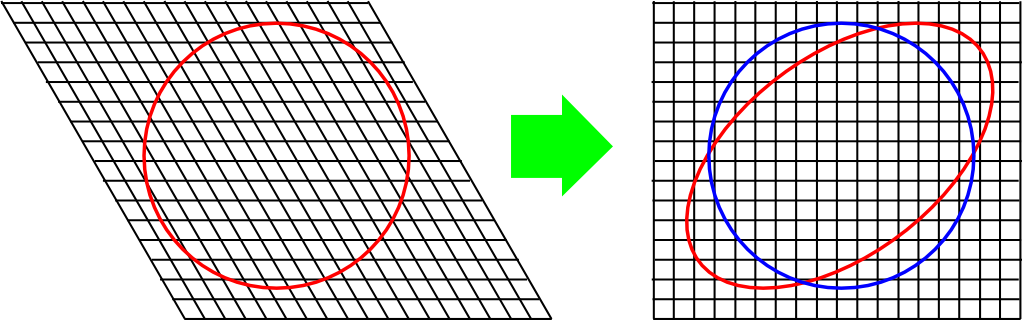
\includegraphics[width=0.8\textwidth]{\figurepath/automation/pulay_stress.png} 
\caption{Demonstration of the influence of a change in lattice vectors on the 
effective energy cutoff. When the lattice changes from hexagonal (left) to a 
cubic (right), the corresponding energy cutoff surface changes from a sphere 
to an ellipsoid, effectively reducing the cutoff energy of the corresponding 
basis set. Taken from~\cite{Pulay}.} 
\label{automation:fig-pulay} 
\end{figure} 
 
A common way of dealing with this issue is to perform an additional geometry 
optimization, as the basis set is initialized again at the start of this 
secondary calculation. However, if the lattice vectors change significantly 
during this second geometry optimization, the same problem might repeat 
itself. \code{PulayTask} tries to deal with this problem automatically by 
checking a user-specified condition versus a certain tolerance, and running 
the geometry optimization again in case this condition is not met. If the 
condition is met, the workflow continues as it was initially 
designed\footnote{In the context of the Fireworks lingo, \code{PulayTask} 
returns an \code{FWAction} that adds the next geometry optimization as an 
\code{addition}.}. If not, another geometry optimization is performed based on 
the final structure. 
 
\subsection{\texttt{ConfigurationTask}/\texttt{EnergyConfTask}} 
\label{automation:sec-ConfigurationTask} \label{automation:sec-EnergyConfTask} 
 
These two tasks make up the complete configuration 
workflow~\ref{automation:sec-configurations}, which can be used to calculate the 
energy of a large set of configurations for any system with degrees of configurational 
freedom in the placement of atoms on specified sites (e.g. 
\link{batteries:sec-structure}{lithium configurations of a charged cathode}).
\code{ConfigurationTask} generates the requested configurations based on the 
algorithm of Hart et al.~\cite{Hart2005} for the provided structure and a 
number of user-specified settings: 
 
\begin{itemize} 
\item \code{substitution\_sites (list)}: Sites of the structure which should 
be considered for substitution. 
\item \code{element\_list (list)}: Which elements are substituted into the 
structure to generate the configurations. 
\item \code{size (list)} : A list of allowed unit cell sizes for generating 
the configurations. Note that the algorithm is able to generate more than just 
supercells. Any unit cell that can reconstruct the structure with a number of 
sites equal to a size in the list times the number of sites in the original 
structure is considered. 
\item \code{concentration\_restrictions (dict)}: Allows the user to specify 
restrictions on the \textit{fractional} concentrations of the elements. 
\end{itemize} 
 
Once the configurations have been generated, \code{EnergyConfTask} sets up a 
two-step workflow for each configuration, consisting of a geometry 
optimization (\code{OptimizeFW}) and a static calculation to obtain a more 
precise value for the energy using the \link{appendix:sec-ISMEAR}{tetrahedron method} (\code{StaticFW}). 
 
\subsection{Other} 
 
Here I give a brief overview of some smaller \code{Firetask}s which are also 
part of the workflows described in Section~\ref{automation:sec-workflows}.  
 
\begin{itemize} 
 
\phantomsection \label{automation:sec-IncreaseNumberOfBands} 
\item \code{IncreaseNumberOfBands}: For some calculations, such as a 
calculation of the dielectric tensor, it is important to have a sufficient 
amount of empty bands. Often, this is done by setting the total number of bands to the number of 
occupied bands from a previous calculation. This \code{Firetask} automates 
this step, based on a user-specified multiplier. 
 
\phantomsection \label{automation:sec-VaspTask} 
\item \code{VaspTask}: Similar to 
\link{automation:sec-CustodianTask}{\code{CustodianTask}}, this 
\code{Firetask} runs VASP in the directory of the \code{Firework}. 
However, this is just a bare VASP run without any error recovery 
based on a \code{Custodian}. In case the user does not specify any 
\code{ErrorHandlers} when initializing a \code{Firework} that runs 
VASP, this class is used instead of \code{CustodianTask}. 
 
\phantomsection \label{automation:sec-NWChemTask} 
\item \code{NWChemTask}: \code{Firetask} that runs an 
\href{http://www.nwchem-sw.org/index.php/Main_Page}{NWChem} calculation in 
the specified directory. This is exclusively used for the calculation of the 
cation energy landscapes around polyborate anions, see Sections~\ref{automation:sec-landscape} and~\ref{batteries:sec-landscape}.
 
\phantomsection \label{automation:sec-AddFinalGeometryToSpec} 
\item \code{AddFinalGeometryToSpec}: This small but handy \code{Firework} 
extracts the final geometry from the current directory and adds it to the 
\code{\_fw\_spec}, so it can be used by both other \code{Firetask}s in the 
\code{Firework}, as well as future \code{Firework}s. 
 
\phantomsection \label{automation:sec-ScriptTask} 
\item \code{ScriptTask}: This is a standard task included in the Fireworks package 
which runs a user-defined command line script. 
 
\phantomsection \label{automation:sec-PyTask} 
\item \code{PyTask}: Versatile task included in Fireworks package that can run 
any Python method. Note that the method is defined as the string which would 
be used to import that method in a Python module, e.g. 
\code{pybat.workflow.workflows.get\_wfs\_noneq\_dimers}. In case a 
\code{PyTask} is used in my workflows, the flowchart will detail the Python 
method used as well as a short explanation. 

\end{itemize} 
 
\section{Workflows} \label{automation:sec-workflows} 
 
In this section I present an overview of the workflows used to calculate the 
results presented in the rest of my thesis. As mentioned previously, all of 
these workflows consist of several \code{Firework}s, each of which represent 
one VASP calculation. As these \code{Firework}s are largely just a 
collection of \code{Firetask}s, I won't describe them separately. It should be 
clear from the description of the workflow what each \code{Firework} does. 
 
\resultsubsection{Optical properties \label{automation:sec-optics}}{https://github.com/mbercx/phd-thesis/tree/master/jupyter/automation\#optical-properties}{} 
 
Section \ref{dft:sec-linear} describes the theoretical framework for 
calculating the electromagnetic response of a material. Here I explain the 
practical steps you have to take to calculate the frequency dependent 
dielectric tensor for any given material, which have been employed to 
calculate the optical properties used in Chapter~\ref{chapter:slme}. As the 
number of steps required here is rather limited, it is an ideal problem to 
demonstrate a simple workflow. 
 
\begin{figure}[ht] 
\begin{tikzpicture}[scale=1, node distance=0.4em]

    % Fireworks
    \node (title_1) [firework_name] {OptimizeFW};
    \node (fw1_1) [firetask, below=of title_1] {\firetask{WriteVaspFromIOSet}};
    \node (fw1_2) [firetask, below=of fw1_1] {\firetask{VaspParallelizationTask}
    };
    \node (fw1_3) [firetask, below=of fw1_2] {
        \firetask{CustodianTask}/\firetask{VaspTask}
    };
    \node (fw1_4) [firetask, below=of fw1_3] {\firetask{AddFinalGeometryToSpec}};
    \node (fw1_5) [firetask, below=of fw1_4] {\firetask{PulayTask}};
    \begin{scope}[on background layer]
        \node (frame_1) [firework, fit={(title_1) (fw1_1) (fw1_2) (fw1_3) (fw1_4) (fw1_5)}] {}; 
    \end{scope}
    
    \node (title_2) [firework_name, below right=2em and 1em of frame_1] {PulayStep};
    \node (fw2_1) [firetask, below=of title_2] {\firetask{ScriptTask}};
    \node (fw2_2) [firetask, below=of fw2_1] {
        \firetask{CustodianTask}/\firetask{VaspTask}
    };
    \node (fw2_3) [firetask, below=of fw2_2] {\firetask{AddFinalGeometryToSpec}};
    \node (fw2_4) [firetask, below=of fw2_3] {\firetask{PulayTask}};
    \begin{scope}[on background layer]
    \node (frame_2)[firework, fit={(title_2) (fw2_1) (fw2_2) (fw2_3) (fw2_4)}] {};
    \end{scope}
    
    \node (title_3) [firework_name, below=14em of frame_1] {OpticsFW};
    \node (fw3_1) [firetask, below=of title_3] {\firetask{WriteVaspFromIOSet}};
    \node (fw3_2) [firetask, below=of fw3_1] {\firetask{VaspParallelizationTask}};
    \node (fw3_3) [firetask, below=of fw3_2] {\firetask{IncreaseNumberOfBands}};
    \node (fw3_4) [firetask, below=of fw3_3] {\firetask{CustodianTask}/\firetask{VaspTask}};
    \node (fw3_5) [firetask, below=of fw3_4] {\firetask{AddFinalGeometryToSpec}};
    \begin{scope}[on background layer]
    \node (frame_3)[firework, fit={(title_3) (fw3_1) (fw3_2) (fw3_3) (fw3_4) (fw3_5)}] {};
    \end{scope}
    
    % Connections
    \draw [->, firearrow] (fw1_5.east) -- (fw1_5.east -| frame_2.north) -- (frame_2.north);
    \draw [->, firearrow] ($(fw1_5.south) - (1em, 0)$) -- node [conditionbox, rotate=90, midway, above left=5em and 0em] {\texttt{condition $<$ tolerance}} ($(frame_3.north) - (1em, 0)$);
    \draw [->, firearrow] (fw2_4.west) -- ($(fw2_4.west) - (4em, 0)$) -- ($(fw2_1.west) - (4em, 0)$) -- (fw2_1.west);
    \draw [->, firearrow] (frame_2.south) -- (frame_2.south |- frame_3.east) -- (frame_3.east);
    
    % Help boxes
    \node (help1)[wf-helpbox, right=3 em of fw1_1] {Write the input files for VASP, based on the Set that defines the calculation.};
    \draw [wf-helpline] (fw1_1.east) -- (help1.west);
    \node (help2)[wf-helpbox, left=3 em of fw1_1] {Trial run of VASP to determine number of irreducible k-points, then configure the parallelization settings.};
    \draw [wf-helpline] (fw1_2.west) -- (fw1_2.west -| help2.east);
    \node (help3)[wf-helpbox, right=5 em of fw1_4, text width=10 em] {Store the full geometry for future fireworks.};
    \draw [wf-helpline] (fw1_4.east) -- (help3.west);
    \node (help4)[wf-helpbox, left=5em of fw1_5, text width=12 em] {Check the change in lattice vectors, perform another \\ geometry optimization in case the change is significant.};
    \draw [wf-helpline] (help4.east) -- (fw1_5.west); 
    \node (help5)[wf-helpbox, left=4em of fw3_3, text width=12 em] {Increase the number of bands to a multiple of the VASP default.};
    \draw [wf-helpline] (help5.east) -- (fw3_3.west); 
    \node (help6)[wf-helpbox, below right=2em and -3em of frame_2, text width=10 em] {Simple bash script that copies the \vasp{CONTCAR} to the \vasp{POSCAR}.};
    \draw [wf-helpline] (help6.north) -- (help6.north |- fw2_1.east) -- (fw2_1.east); 
   
\end{tikzpicture}
 
\caption{\label{automation:fig-optics} Flowchart for the optics workflow.} 
\end{figure} 
 
Figure~\ref{automation:fig-optics} shows the workflow applied to each 
structure. As the unit is often constructed by replacing elements in a 
template of the unit cell with the required spacegroup, the first step is to 
optimize the geometry of the structure\footnote{Note that in case a 
\link{dft:sec-hybrid}{hybrid functional} is used, it is efficient to first 
optimize the geometry using a less computationally demanding functional, 
especially when we generate structures that might have very different lattice 
parameters than the final structure.} in the \code{OptimizeFW}. Here we allow 
for a full optimization of the unit cell (\vasp{ISIF}~=~3), and as such the 
lattice vectors can change. In case the energy of the initial structure and 
final structure differs more than 1~\si{\milli\electronvolt} per atom, the 
\link{automation:sec-PulayTask}{\code{PulayTask}} copies the final structure 
\vasp{CONTCAR} to the \vasp{POSCAR} and performs another geometry optimization 
in a \code{PulayStep}. 
 
Once the geometry is obtained, the workflow continues by calculating the 
dielectric tensor in the \code{OpticsFW}. This requires an increase in the 
number of bands, as to have enough unoccupied bands to calculate the 
\link{dft:sec-dielectric}{dielectric tensor} for sufficiently high energy 
transitions. Besides this, the \code{OpticsFW} also configures some default 
settings for dielectric function calculations, e.g. \vasp{LOPTICS}=True, a 
more dense energy grid (\vasp{NEDOS}=2000) and a more strict electronic 
convergence criterion (\vasp{EDIFF}=$10^{-6}$). Finally, the \code{Firework} 
also sets the \vasp{CSHIFT} parameter to 0.01, which should be sufficiently low to make sure 
that VASP does not overwrite the original imaginary part of the 
dielectric tensor with the one obtained from the Kramers-Kronig relation (See Appendix~\ref{appendix:sec-cshift}). This 
introduces a broadening to the imaginary part of the dielectric tensor, which 
is passed to the absorption coefficient through 
Eq.~(\ref{slme:eq-absorption}). In effect, this reduces the band gap of the 
material, which has a large influence on the calculated efficiency described 
in Section~\ref{slme:sec-efficiency}. 
 
\resultsubsection{Configurations \label{automation:sec-configurations}}{https://github.com/mbercx/phd-thesis/tree/master/jupyter/automation\#configurations}{} 
 
For various research questions, it is important to be able to investigate a 
whole range of configurations for a specific property. For example, when 
investigating the structural stability of a charged battery cathode, it is 
important to consider the most stable lithium 
configuration (Sec.~\ref{batteries:sec-structure}). 
Figure~\ref{automation:fig-configurations} shows the configuration workflow, 
which at first only consists of a single \code{Firework} that generates all 
configurations for a specified set of restrictions using the algorithm of Hart 
et al.~\cite{Hart2005}, as implemented in 
\link{automation:sec-ConfigurationTask}{\code{ConfigurationTask}}. The 
resulting list of symmetrically non-equivalent configurations is passed to the 
\link{automation:sec-EnergyConfTask}{\code{EnergyConfTask}}, which sets up a 
\code{Workflow} that optimizes the geometry of each configuration and 
subsequently determines the total energy based on a static calculation. 
 
\begin{figure}[ht] 
\centering 
\begin{tikzpicture}[scale=1, node distance=0.4em]

% Fireworks
\node (conf) [font=\bf\ttfamily] {ConfigurationFW};
\node (conf_1) [firetask, below=of conf] {\firetask{ConfigurationTask}};
\node (conf_2) [firetask, below=of conf_1] {\firetask{EnergyConfTask}};
\begin{scope}[on background layer]
    \node (frame_conf) [firework, fit={(conf) (conf_1) (conf_2)}] {};
\end{scope}

\node (energy_wf0) [firetask, align=center, thick, rounded corners, below left= 3em and 5 em of frame_conf] {configuration\_0 \\ energy workflow};
\node (energy_wf1) [firetask, align=center, thick, rounded corners, right= 3em of energy_wf0] {configuration\_1 \\ energy workflow};
\node (energy_wf_dot) [firetask, align=center, thick, rounded corners, right= 3em of energy_wf1] {...};
\node (energy_wfn) [firetask, align=center, thick, rounded corners, right= 3em of energy_wf_dot] {configuration\_n \\ energy workflow};

\node (optimize) [font=\bf\ttfamily, below=7em of energy_wf0] {OptimizeFW};
\node (optimize_1) [firetask, below=of optimize] {\firetask{WriteVaspFromIOSet}};
\node (optimize_2) [firetask, below=of optimize_1] {\firetask{VaspParallelizationTask}};
\node (optimize_3) [firetask, below=of optimize_2] {\firetask{CustodianTask}/\firetask{VaspTask}};
\node (optimize_4) [firetask, below=of optimize_3] {\firetask{AddFinalGeometryToSpec}};
\node (optimize_5) [firetask, below=of optimize_4] {\firetask{PulayTask}};
\begin{scope}[on background layer]
    \node (frame_optimize) [firework, fit={(optimize) (optimize_1) (optimize_2) (optimize_3) (optimize_4) (optimize_5)}] {}; 
\end{scope}

\node (pulay) [font=\bf\ttfamily, above right=2em and 5em of frame_optimize] {\firetask{PulayStep}};
\node (pulay_1) [firetask, below=of pulay] {\firetask{ScriptTask}};
\node (pulay_2) [firetask, below=of pulay_1] {\firetask{CustodianTask}/\firetask{VaspTask}};
\node (pulay_3) [firetask, below=of pulay_2] {\firetask{AddFinalGeometryToSpec}};
\node (pulay_4) [firetask, below=of pulay_3] {\firetask{PulayTask}};
\begin{scope}[on background layer]
\node (frame_pulay)[firework, fit={(pulay) (pulay_1) (pulay_2) (pulay_3) (pulay_4)}] {};
\end{scope}

\node (static) [font=\bf\ttfamily, right=19em of optimize_1] {StaticFW};
\node (static_1) [firetask, below=of static] {\firetask{WriteVaspFromIOSet}};
\node (static_2) [firetask, below=of static_1] {\firetask{VaspParallelizationTask}};
\node (static_3) [firetask, below=of static_2] {\firetask{CustodianTask}/\firetask{VaspTask}};
\node (static_4) [firetask, below=of static_3] {\firetask{AddFinalGeometryToSpec}};
\begin{scope}[on background layer]
\node (frame_static)[firework, fit={(static) (static_1) (static_2) (static_3) (static_4)}] {};
\end{scope}

% Connections
\coordinate (conf_split) at ($(frame_conf.south) + (0, -1.5em)$);
\draw [->, firearrow, solid] (conf_2.south) -- (conf_split) -- (conf_split -| energy_wf0.north) -- (energy_wf0.north);
\draw [->, firearrow, solid] (conf_split) -- (conf_split -| energy_wf1.north) -- (energy_wf1.north);
\draw [->, firearrow, solid] (conf_split) -- (conf_split -| energy_wf_dot.north) -- (energy_wf_dot.north);
\draw [->, firearrow, solid] (conf_split) -- (conf_split -| energy_wfn.north) -- (energy_wfn.north);

\coordinate (pulay_merge) at ($(pulay_4.west) - (4em, 3em)$);
\draw [->, firearrow] (optimize_5.east) -- node [conditionbox, midway, above right=0em and -3em] {\texttt{condition $<$ tolerance}} (optimize_5.east -| frame_static.west);
\draw [->, firearrow] (optimize_5.east -| pulay_merge) -- (pulay_merge);
\draw [firearrow] (pulay_merge) -- ($(pulay_4.west) - (4em, 0em)$);
\draw [->, firearrow] (pulay_4.west) -- ($(pulay_4.west) - (4em, 0em)$);
\draw [->, firearrow] (pulay_merge) -- ($(pulay_1.west) - (4em, 0)$) -- (pulay_1.west);
\draw [->, firearrow] (pulay_4.east) -- (pulay_4.east -| frame_static.west);

% Help boxes

\node (help1)[helpbox, right=3 em of conf_1] {Generates configurations based on user specifications.};
\draw [helpline] (conf_1.east) -- (help1.west);
\node (help2)[helpbox, left=3 em of conf_2] {Sets up an energy workflow for each configuration.};
\draw [helpline] (conf_2.west) -- (help2.east);
\node (help2)[helpbox, text width=13.5em, above right=2 em and -6em of frame_static.north] {The \texttt{StaticFW}  determines the energy with higher precision using the tetrahedron method.};
\draw [helpline] (frame_static.north) -- (frame_static.north |- help2.south);

% Frame for energy workflow
\node (frame_wf_energy)[draw, thick, rounded corners, inner sep=1 em, fit={(frame_optimize) (frame_pulay) (frame_static) (help2)}] {};
\draw [thick] (energy_wf0.south) -- (energy_wf0.south |- frame_wf_energy.north);

\end{tikzpicture} 
\caption{\label{automation:fig-configurations} Flowchart for the 
configurations workflow.} 
\end{figure} 
 
\resultsubsection{Kinetic barriers - dimer workflow \label{automation:sec-dimer}}{https://github.com/mbercx/phd-thesis/tree/master/jupyter/automation\#kinetic-barriers---dimer-workflow}{}  
 
As explained in Section~\ref{dft:sec-transition}, investigating a transition 
from one state of a system to another requires the calculation of both 
reaction energy and the kinetic barrier. After optimizing the geometry of two 
different states of a material, we can compare their energies in order to get 
an idea of the thermodynamic driving force for the transition. If such a 
reaction is favorable, i.e. its reaction energy is found to be negative, we 
still have to make sure that the transition is kinetically feasible. One 
method for doing this is calculating the kinetic barrier directly using the 
\link{dft:sec-neb}{nudged elastic band method}. 
 
\begin{figure}[ht!] 
\centering 
\begin{tikzpicture}[scale=1, node distance=0.4em]

% Fireworks
\node (optimize) [font=\bf\ttfamily] {OptimizeFW};
\node (optimize_1) [firetask, below=of optimize] {\firetask{WriteVaspFromIOSet}};
\node (optimize_2) [firetask, below=of optimize_1] {\firetask{VaspParallelizationTask}};
\node (optimize_3) [firetask, below=of optimize_2] {\firetask{CustodianTask}/\firetask{VaspTask}};
\node (optimize_4) [firetask, below=of optimize_3] {\firetask{AddFinalGeometryToSpec}};
\node (optimize_5) [firetask, below=of optimize_4] {\firetask{PulayTask}};
\begin{scope}[on background layer]
    \node (frame_optimize) [firework, fit={(optimize) (optimize_1) (optimize_2) (optimize_3) (optimize_4) (optimize_5)}] {}; 
\end{scope}

\node (pulay) [font=\bf\ttfamily, below=3em of frame_optimize] {\firetask{PulayStep}};
\node (pulay_1) [firetask, below=of pulay] {\firetask{ScriptTask}};
\node (pulay_2) [firetask, below=of pulay_1] {\firetask{CustodianTask}/\firetask{VaspTask}};
\node (pulay_3) [firetask, below=of pulay_2] {\firetask{AddFinalGeometryToSpec}};
\node (pulay_4) [firetask, below=of pulay_3] {\firetask{PulayTask}};
\begin{scope}[on background layer]
\node (frame_pulay)[firework, fit={(pulay) (pulay_1) (pulay_2) (pulay_3) (pulay_4)}] {};
\end{scope}

\node (static) [font=\bf\ttfamily, right=8em of pulay] {StaticFW};
\node (static_1) [firetask, below=of static] {\firetask{WriteVaspFromIOSet}};
\node (static_2) [firetask, below=of static_1] {\firetask{VaspParallelizationTask}};
\node (static_3) [firetask, below=of static_2] {\firetask{CustodianTask}/\firetask{VaspTask}};
\node (static_4) [firetask, below=of static_3] {\firetask{AddFinalGeometryToSpec}};
\begin{scope}[on background layer]
\node (frame_static)[firework, fit={(static) (static_1) (static_2) (static_3) (static_4)}] {};
\end{scope}

\node (dimer) [font=\bf\ttfamily, right=4em of frame_static] {DimerFW};
\node (dimer_1) [firetask, below=of dimer] {\firetask{PyTask}};
\begin{scope}[on background layer]
    \node (frame_dimer) [firework, fit={(dimer) (dimer_1)}] {};
\end{scope}

\node (energy_wfn) [firetask, align=center, thick, rounded corners, below=5em of frame_dimer] {dimer (O$_a^n$, O$_b^n$) \\ transition workflow};
\node (energy_wf_dot) [firetask, align=center, thick, rounded corners, left= 3em of energy_wfn] {...};
\node (energy_wf1) [firetask, align=center, thick, rounded corners, left= 3em of energy_wf_dot] {dimer (O$_a^1$, O$_b^1$) \\ transition workflow};
\node (energy_wf0) [firetask, align=center, thick, rounded corners, left=3em of energy_wf1] {dimer (O$_a^0$, O$_b^0$) \\ transition workflow};

\node (trans_opt) [font=\bf\ttfamily, below right=3em and -2em of energy_wf0] {OptimizeFW};
\node (trans_opt_1) [firetask, below=of trans_opt] {\firetask{WriteVaspFromIOSet}};
\node (trans_opt_2) [firetask, below=of trans_opt_1] {\firetask{VaspParallelizationTask}};
\node (trans_opt_3) [firetask, below=of trans_opt_2] {\firetask{CustodianTask}/\firetask{VaspTask}};
\node (trans_opt_4) [firetask, below=of trans_opt_3] {\firetask{AddFinalGeometryToSpec}};
\begin{scope}[on background layer]
    \node (frame_trans_opt) [firework, fit={(trans_opt) (trans_opt_1) (trans_opt_2) (trans_opt_3) (trans_opt_4)}] {}; 
\end{scope}

\node (trans_static) [font=\bf\ttfamily, right=10em of trans_opt] {StaticFW};
\node (trans_static_1) [firetask, below=of trans_static] {\firetask{WriteVaspFromIOSet}};
\node (trans_static_2) [firetask, below=of trans_static_1] {\firetask{VaspParallelizationTask}};
\node (trans_static_3) [firetask, below=of trans_static_2] {\firetask{CustodianTask}/\firetask{VaspTask}};
\node (trans_static_4) [firetask, below=of trans_static_3] {\firetask{AddFinalGeometryToSpec}};
\begin{scope}[on background layer]
\node (frame_trans_static)[firework, fit={(trans_static) (trans_static_1) (trans_static_2) (trans_static_3) (trans_static_4)}] {};
\end{scope}

\node (neb) [font=\bf\ttfamily, below left=4em and 10em of frame_trans_static] {NebFW};
\node (neb_1) [firetask, below=of neb] {\firetask{WriteVaspFromIOSet}};
\node (neb_2) [firetask, below=of neb_1] {\firetask{VaspParallelizationTask}};
\node (neb_3) [firetask, below=of neb_2] {\firetask{CustodianTask}/\firetask{VaspTask}};
\node (neb_4) [firetask, below=of neb_3] {\firetask{AddFinalGeometryToSpec}};
\begin{scope}[on background layer]
\node (frame_neb)[firework, fit={(neb) (neb_1) (neb_2) (neb_3) (neb_4)}] {};
\end{scope}

\node (postprocess) [font=\bf\ttfamily, below=4em of frame_trans_static] {PostProcessFW};
\node (postprocess_1) [firetask, below=of postprocess] {\firetask{PyTask}};
\begin{scope}[on background layer]
\node (frame_postprocess)[firework, fit={(postprocess) (postprocess_1)}] {};
\end{scope}

% Connections
\draw [->, firearrow] (optimize_5.south) -- (frame_pulay.north);
\draw [->, firearrow] (optimize_5.east) -- node [conditionbox, above right=0em and -1em] {\texttt{condition $<$ tolerance}} (optimize_5.east -| frame_static.north) -- (frame_static.north);
\draw [->, firearrow] (pulay_4.west) -- ($(pulay_4.west) - (4em, 0)$) -- ($(pulay_1.west) - (4em, 0)$) -- (pulay_1.west);
\draw [->, firearrow] (pulay_4.east) -- (pulay_4.east -| frame_static.west);
\draw [->, firearrow] (frame_static.east |- frame_dimer.west) -- (frame_dimer.west);

\coordinate (conf_split) at ($(frame_dimer.south) + (0, -3.5em)$);
\draw [->, firearrow, solid] (dimer_1.south) -- (conf_split) -- (conf_split -| energy_wf0.north) -- (energy_wf0.north);
\draw [->, firearrow, solid] (conf_split) -- (conf_split -| energy_wf1.north) -- (energy_wf1.north);
\draw [->, firearrow, solid] (conf_split) -- (conf_split -| energy_wf_dot.north) -- (energy_wf_dot.north);
\draw [->, firearrow, solid] (conf_split) -- (conf_split -| energy_wfn.north) -- (energy_wfn.north);

\coordinate (neb_split) at ($(frame_trans_static.south) + (0, -2em)$);
\draw [->, firearrow] (frame_trans_opt.east) -- (frame_trans_static.west);
\draw [->, firearrow] (frame_trans_static.south) -- (neb_split) -- node [conditionbox, midway, above] {\texttt{reaction\_energy $<$ tolerance}} (neb_split -| frame_neb) -- (frame_neb.north);
\draw [->, firearrow] (neb_split) -- (frame_postprocess.north);
\draw [->, firearrow] (frame_neb.east |- frame_postprocess.west) -- (frame_postprocess.west);

% % Help boxes

\node (help1)[helpbox, text width=22em, above left=10 em and -8em of frame_dimer] {
\texttt{get\_wfs\_noneq\_dimers(structure, distance, ...):} \\ 
\textit{\begin{tabular}{l l}
& Set up a transition workflow for each of the \\
& non-equivalent dimers of \texttt{structure}. The dimer \\
& is constructured by pushing the pair of oxygen \\
& atoms closer, to \texttt{distance}.
\end{tabular}}
};
\coordinate (help1_line) at ($(dimer_1.east) + (1em, 0em)$);
\draw [helpline] (dimer_1.east) -- (help1_line) -- (help1_line |- help1.south);

\node (help2)[helpbox, text width=19em, below left=2 em and -14em of frame_postprocess] {
\texttt{post\_process\_dimer\_neb(directory, ...):} \\ 
\textit{\begin{tabular}{l l}
& Check the output in \texttt{directory} and either \\
& simply extract the energies and structures \\
& or use the \texttt{DimerNebAnalysis} class to set \\ 
& up the NEB data file. \\
\end{tabular}}
};
\coordinate (help1_line) at ($(dimer_1.east) + (1em, 0em)$);
\draw [helpline] (postprocess_1.south) -- (postprocess_1.south |- help2.north);

% Frame for energy workflow
\node (frame_wf_energy)[draw, thick, rounded corners, inner sep=1 em, fit={(frame_trans_opt) (frame_neb) (frame_trans_static) (help2)}] {};
\draw [firearrow, solid] (energy_wf0.south) -- (energy_wf0.south |- frame_wf_energy.north) -- (frame_wf_energy);

\end{tikzpicture} 
\caption{\label{automation:fig-dimer} Flowchart for the dimer workflow.} 
\end{figure} 
 
The investigation of the stability of the oxygen framework presented in 
Section~\ref{batteries:sec-dimer} requires the thermodynamics and kinetics of 
oxygen dimer formation. Figure~\ref{automation:fig-dimer} shows the workflow 
that executes the necessary steps. First, the geometry of the provided 
structure is fully optimized (\vasp{ISIF}=3), and the energy is calculated 
more precisely using a static calculation. The final structure and energy is 
passed on to a small \code{Firework} that sets up a transition workflow
for each non-equivalent dimer. This transition work flow consists of a 
geometry optimization of the dimer structure, where only the atomic positions 
are allowed to optimize (\vasp{ISIF}=2. Once again a static calculation is 
performed to determine the energy, which is then compared to the energy of the 
initial, unperturbed structure in order to obtain the reaction energy. If this 
reaction energy is smaller than a certain tolerance\footnote{Note that the reaction energy is defined as the final energy minus the initial energy. Hence, a transition with a negative reaction energy is thermodynamically favorable, i.e. setting the \code{tolerance} to zero only calculates the kinetic barrier for thermodynamically favorable dimers.}, the kinetic barrier is 
calculated using a \link{dft:sec-neb}{nudged elastic band calculation}. 

\resultsubsection{Landscapes \label{automation:sec-landscape}}{https://github.com/mbercx/phd-thesis/tree/master/jupyter/automation\#landscapes}{} 

The energy landscapes presented in Section~\ref{batteries:sec-landscape} require 
knowledge about the energy of the anion-cation system for a range of cation 
positions on a two dimensional surface. We represent the landscape as a grid of 
points or coordinates, for which we determine the energy of the system with a 
static DFT calculation. Although it is possible to simulate molecules in VASP 
-- despite its use of three dimensional periodic boundary conditions -- by 
considering a large unit cell, we choose to use 
\href{http://www.nwchem-sw.org/index.php/Main_Page}{NWChem}~\cite{Valiev2010}. 
This software package is more suitable for the study of molecules as it does 
not enforce the use of periodic boundary conditions. 

\begin{figure}[ht] 
\begin{tikzpicture}


\node (chain_setup) [wf-helpbox, text width=18em, anchor=west, font=\footnotesize] at (-8, 0) {
\texttt{\textbf{chain\_setup}(filename, cation, facets, ...):} \\ 
\textit{\begin{tabular}{l l}
& Set up a \texttt{cation} landscape for 2D wedges \\
& along a chain of \texttt{facets} for the molecule \\
& stored in \texttt{filename}.
\end{tabular}}
};

\node (sphere_setup) [wf-helpbox, text width=18em, anchor=east, font=\footnotesize] at (8, 0) {
\texttt{\textbf{sphere\_setup}(filename, cation, radius, ...):} \\ 
\textit{\begin{tabular}{l l}
& Set up a \texttt{cation} landscape for a sphere \\
& with a specified \texttt{radius} for the molecule \\
& stored in \texttt{filename}.
\end{tabular}}
};

\node (chain) [below=13.2em of chain_setup.west, anchor=west] {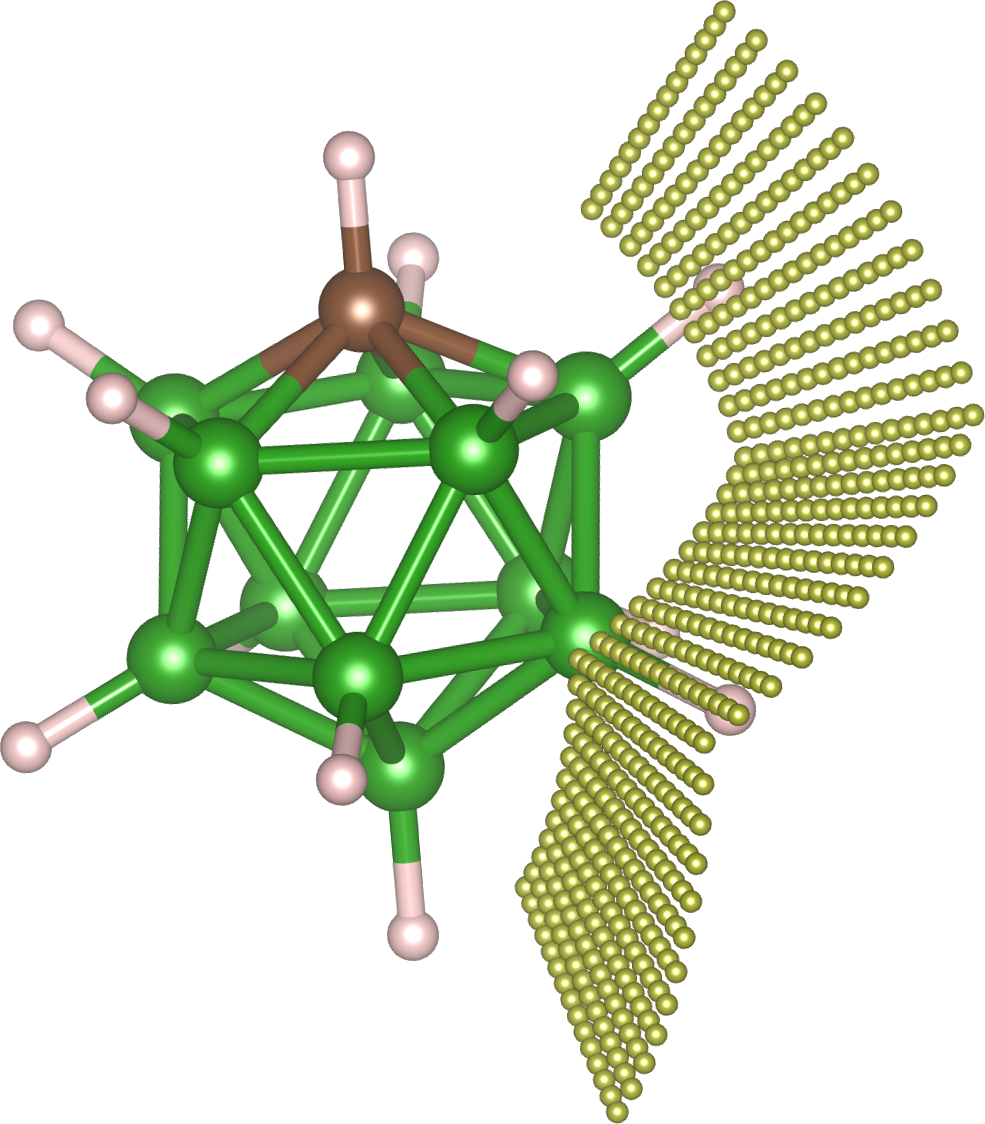
\includegraphics[width=140px]{\figurepath/automation/chain_landscape.png}};

\node (sphere) [below=13em of sphere_setup.east, anchor=east] {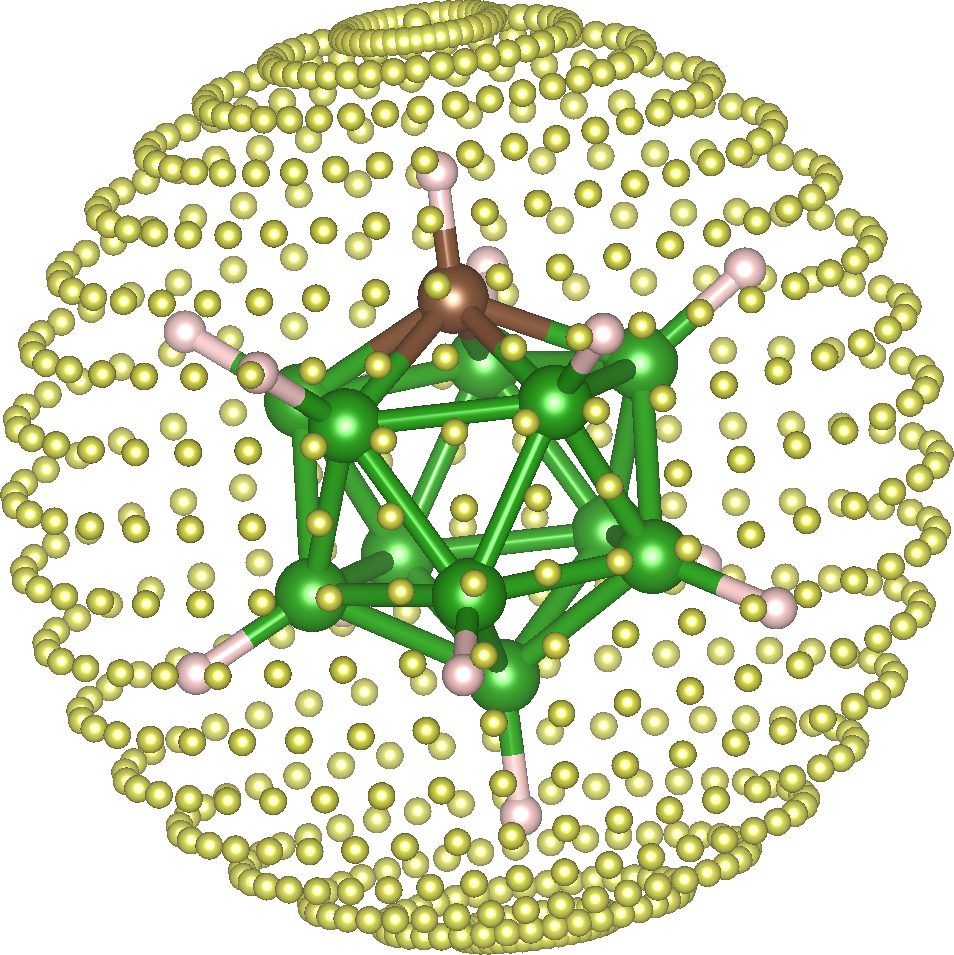
\includegraphics[width=150px]{\figurepath/automation/sphere_landscape.png}};

% Fireworks
\node (title_static1) [firework_name] at (0, -2) {StaticFW};
\node (static1_1) [firetask, below=0.2 em of title_static1] {\firetask{NWChemTask}};
\node (static1_2) [firetask, below=0.2 em of static1_1] {\firetask{ScriptTask}};

\begin{scope}[on background layer]
\node (frame_static1) [firework, fit={(title_static1) (static1_1) (static1_2)}] {}; 
\end{scope}

% Fireworks
\node (title_static2) [firework_name, below=1em of frame_static1] {StaticFW};
\node (static2_1) [firetask, below=0.2 em of title_static2] {\firetask{NWChemTask}};
\node (static2_2) [firetask, below=0.2 em of static2_1] {\firetask{ScriptTask}};

\begin{scope}[on background layer]
\node (frame_static2) [firework, fit={(title_static2) (static2_1) (static2_2)}] {}; 
\end{scope}

\node (dots) [below=1em of frame_static2] {...};

% Fireworks
\node (title_static3) [firework_name, below=1em of dots] {StaticFW};
\node (static3_1) [firetask, below=0.2 em of title_static3] {\firetask{NWChemTask}};
\node (static3_2) [firetask, below=0.2 em of static3_1] {\firetask{ScriptTask}};

\begin{scope}[on background layer]
\node (frame_static3) [firework, fit={(title_static3) (static3_1) (static3_2)}] {}; 
\end{scope}

\node (frame_wf) [draw, thick, rounded corners, fit={(frame_static1) (frame_static2) (frame_static3)}] {}; 

\draw [thick] ($(frame_wf.east) + (0, 6em)$) -- ($(frame_wf.east) + (5em, 6em)$);
\draw [thick] ($(frame_wf.west) + (0, 6em)$) -- ($(frame_wf.west) + (-5.5em, 6em)$);

\node (process_output) [wf-helpbox, text width=16em, below=26.5em of sphere_setup.east, anchor=east, font=\footnotesize] {
\texttt{\textbf{process\_output}(output\_path):} \\ 
\textit{\begin{tabular}{l l}
& Check the output in \texttt{output\_path}, \\ 
& load it in the \texttt{NwOutput} class\\
& and write it to a \texttt{.json} file. \\ 
\end{tabular}}
};

\node (helpbox1) [wf-helpbox, text width=14em, below=25em of chain_setup.west, anchor=west, font=\footnotesize] {
For each point in the energy landscape, a static calculation (\texttt{StaticFW}) is added to the workflow.
};

\coordinate (help1_bend) at ($(chain_setup.east) + (1em, 0em)$);
\draw [wf-helpline, ->, >=latex] (chain_setup.south) -- (chain.north -| chain_setup.south);
\draw [wf-helpline, ->, >=latex] (chain_setup.east) -- (help1_bend) -- (help1_bend |- frame_wf.north);
\coordinate (help2_bend) at ($(sphere_setup.west) + (-1em, 0em)$);
\draw [wf-helpline, ->, >=latex] (sphere_setup.south) -- (chain.north -| sphere_setup.south);
\draw [wf-helpline, ->, >=latex] (sphere_setup.west) -- (help2_bend) -- (help2_bend |- frame_wf.north);

\draw [wf-helpline] (static3_2.east) -- (static3_2.east -| process_output.north) -- (process_output.north);

\coordinate (help3_bend) at ($(helpbox1.north) + (6em, 5em)$);

\draw [wf-helpline] (helpbox1.north -| help3_bend) -- (help3_bend) -- (help3_bend -| frame_wf.west) ;

\end{tikzpicture}

 
\caption{Flowchart for the landscape workflow.} 
\label{automation:fig-landscape} 
\end{figure} 

The landscape workflows, shown schematically in Fig.~\ref{automation:fig-landscape}, 
rely on two setup scripts, \code{setup\_chain} and \code{setup\_sphere}, which 
initialize the \code{Landscape} according to the parameters specified by the 
user. For each coordinate in the landscape grid, a static calculation is added 
to the workflow, followed by a small \code{ScriptTask} that processes the output 
from the NWchem output file into a more succinct \code{.json} file. The data for
each segment of the landscape is then mapped back onto the landscape using the 
\code{LandscapeAnalyzer} class, and subsequently tied together. Note that a single 
landscape can consist of hundreds or even thousands of grid points, which makes 
its calculation impractical without the use of a workflow.

\resultsubsection{Surface properties \label{automation:sec-surface}}{https://github.com/mbercx/phd-thesis/tree/master/jupyter/automation\#surface-properties}{}  
 
The calculation of the secondary electron emission in the QUOTAS project 
(Chapter \ref{chapter:quotas}) requires the DOS of the surface states, as well 
as the surface work function. However, because of the three dimensional 
periodic boundary conditions in VASP, simulating an isolated surface 
is not possible. The usual approach for dealing with this issue is by setting 
up a so-called \text{slab} geometry, where we introduce a layer of vacuum to 
the unit cell. In effect, this means that we have \textit{two} opposite 
surfaces in our unit cell, hence the term slab is used instead of surface. 
Moreover, the use of periodic boundary conditions means that we have an 
infinite amount of slabs, but in case the vacuum is chosen to be sufficiently 
thick, the interaction between the surfaces of the slabs is negligible, and we 
can reasonably simulate a surface for the calculation or surface energies, 
work functions and other properties.  
 
Let's describe the process of constructing such a slab unit cell in more 
detail. Usually, the surface is defined based on its Miller indices in the 
conventional unit cell of the bulk structure. However, for many structures, 
there are several possible surfaces corresponding to a set of miller indices, 
depending on where we apply the cleavage plane in the structure. This leads to 
several possible terminations for each set of miller indices. It is good 
practise to consider all terminations for each surface and calculate the 
surface energy to determine the most stable surface, and continue further 
calculations with this termination. Note that this approach does not consider 
the possibility of surface reconstruction. This is a difficult problem to 
solve, as probing all possible surface reconstructions is an insurmountable 
task. Surface reconstruction is especially common for polar surfaces, where 
the ionic nature of the bonds in the structure results in a dipole 
moment across the surface. Tasker~\cite{Tasker1979} distinguished three types 
of ionic surfaces: 
\begin{itemize} 
\item Type I: Individual layers are charge neutral, and hence there is no 
surface dipole. 
\item Type II: Individual layers are charged, but groups of layers can be 
chosen that are charge neutral and non-polar. 
\item Type III: Groups of layers have a net dipole. 
\end{itemize} 
For the work presented in this thesis, I have only performed calculations on 
elemental surfaces, which are always of Tasker Type I and hence non-polar. 
 
Once the surface and its termination have been decided, there are still 
several elements to consider before finalizing the unit cell for the 
calculations. The first thing to specify is the thickness of the slab, i.e. 
the amount of atomic layers, which should be large enough that the center of 
the slab behaves like the bulk of the material under investigation. Second, 
the thickness of the vacuum layer, i.e. the distance between two slabs in the 
periodic boundary conditions, must be set by suitably adjusting the unit cell 
and atom coordinates. In order to make sure both are sufficiently thick, 
convergence of the property of interest versus both slab and vacuum thickness 
should be checked. 
 
The model for secondary electron emission described in 
Section~\ref{quotas:sec-see} requires the density of states and the vacuum level. 
Starting from the bulk structure, the desired surface miller indices need to 
be provided, as well as the \code{slab\_settings}, e.g. the number of 
\code{free\_layers} on each side of the slab. Once the geometry of the bulk 
structure has been fully optimized, the algorithm continues with calculating 
the dielectric tensor using a \code{OpticsFW}. Simultaneously, all 
terminations of the requested surfaces are generated, and a DOS workflow is 
initialized for each resulting slab. Each of these workflows starts with an 
optimization that \textit{relaxes} the surface atoms, depending on how many 
free layers are specified. Finally, the workflow calculates the slab DOS in 
two steps: one run with a sparse k-point mesh in order to obtain a reasonable 
charge density, and one with a dense k-point mesh in order to obtain a precise 
DOS and local potential. 
 
\begin{figure}[ht] 
\begin{tikzpicture}[scale=1, node distance=0.4em]

% Fireworks

\node (optimize) [font=\bf\ttfamily] {OptimizeFW};
\node (optimize_1) [firetask, below=of optimize] {\firetask{WriteVaspFromIOSet}};
\node (optimize_2) [firetask, below=of optimize_1] {\firetask{VaspParallelizationTask}};
\node (optimize_3) [firetask, below=of optimize_2] {\firetask{CustodianTask}/\firetask{VaspTask}};
\node (optimize_4) [firetask, below=of optimize_3] {\firetask{AddFinalGeometryToSpec}};
\node (optimize_5) [firetask, below=of optimize_4] {\firetask{PulayTask}};
\begin{scope}[on background layer]
    \node (optimize_frame) [firework, fit={(optimize) (optimize_1) (optimize_2) (optimize_3) (optimize_4) (optimize_5)}] {}; 
\end{scope}

\node (pulay) [font=\bf\ttfamily, right=6.2em of optimize_3] {\firetask{PulayStep}};
\node (pulay_1) [firetask, below=of pulay] {\firetask{ScriptTask}};
\node (pulay_2) [firetask, below=of pulay_1] {\firetask{CustodianTask}/\firetask{VaspTask}};
\node (pulay_3) [firetask, below=of pulay_2] {\firetask{AddFinalGeometryToSpec}};
\node (pulay_4) [firetask, below=of pulay_3] {\firetask{PulayTask}};
\begin{scope}[on background layer]
\node (pulay_frame)[firework, fit={(pulay) (pulay_1) (pulay_2) (pulay_3) (pulay_4)}] {};
\end{scope}

\node (dos_wf0) [firetask, align=center, thick, rounded corners, below=7em of optimize_frame] {slab\_0 \\ dos workflow};
\node (dos_wf1) [firetask, align=center, thick, rounded corners, right= 3em of dos_wf0] {slab\_1 \\ dos workflow};
\node (dos_wf_dot) [firetask, align=center, thick, rounded corners, right= 3em of dos_wf1] {...};
\node (dos_wfn) [firetask, align=center, thick, rounded corners, right= 3em of dos_wf_dot] {slab\_n \\ dos workflow};

\node (optics) [firework_name, right=22em of optimize] {OpticsFW};
\node (optics_1) [firetask, below=of optics] {\firetask{WriteVaspFromIOSet}};
\node (optics_2) [firetask, below=of optics_1] {\firetask{VaspParallelizationTask}};
\node (optics_3) [firetask, below=of optics_2] {\firetask{IncreaseNumberOfBands}};
\node (optics_4) [firetask, below=of optics_3] {\firetask{CustodianTask}/\firetask{VaspTask}};
\node (optics_5) [firetask, below=of optics_4] {\firetask{AddFinalGeometryToSpec}};
\begin{scope}[on background layer]
\node (optics_frame)[firework, fit={(optics) (optics_1) (optics_2) (optics_3) (optics_4) (optics_5)}] {};
\end{scope}

\node (slab_opt) [font=\bf\ttfamily, below=6em of dos_wf0] {SlabOptimizeFW};
\node (slab_opt_1) [firetask, below=of slab_opt] {\firetask{WriteVaspFromIOSet}};
\node (slab_opt_2) [firetask, below=of slab_opt_1] {\firetask{VaspParallelizationTask}};
\node (slab_opt_3) [firetask, below=of slab_opt_2] {\firetask{CustodianTask}/\firetask{VaspTask}};
\node (slab_opt_4) [firetask, below=of slab_opt_3] {\firetask{AddFinalGeometryToSpec}};
\begin{scope}[on background layer]
\node (slab_opt_frame) [firework, fit={(slab_opt) (slab_opt_1) (slab_opt_2) (slab_opt_3) (slab_opt_4)}] {};
\end{scope}

\node (slab_dos) [font=\bf\ttfamily, above right=1em and 8em of slab_opt] {SlabDosFW};
\node (slab_dos_1) [firetask, below=of slab_dos] {\firetask{WriteVaspFromIOSet}};
\node (slab_dos_2) [firetask, below=of slab_dos_1] {\firetask{VaspParallelizationTask}};
\node (slab_dos_3) [firetask, below=of slab_dos_2] {\firetask{CustodianTask}/\firetask{VaspTask}};
\node (slab_dos_4) [firetask, below=of slab_dos_3] {\firetask{WriteVaspFromIOSet}};
\node (slab_dos_5) [firetask, below=of slab_dos_4] {\firetask{VaspParallelizationTask}};
\node (slab_dos_6) [firetask, below=of slab_dos_5] {\firetask{IncreaseNumberOfBands}};
\node (slab_dos_7) [firetask, below=of slab_dos_6] {\firetask{CustodianTask}/\firetask{VaspTask}};
\node (slab_dos_8) [firetask, below=of slab_dos_7] {\firetask{AddFinalGeometryToSpec}};
\begin{scope}[on background layer]
\node (slab_dos_frame)[firework, fit={(slab_dos) (slab_dos_1) (slab_dos_2) (slab_dos_3) (slab_dos_4) (slab_dos_5) (slab_dos_6) (slab_dos_7) (slab_dos_8)}] {};
\end{scope}

% Connections
\coordinate (pulay_split) at ($(optimize_5.east) + (4em, 0em)$);
\draw [->, firearrow] (optimize_5.east) -- (pulay_frame.west);
\draw [->, firearrow] (pulay_split) -- (pulay_split |- optics_1) -- node [conditionbox, above] {\texttt{condition $<$ tolerance}} (optics_1 -| optics_frame.west);
\draw [->, firearrow] (pulay_4.east) -- (pulay_4.east -| optics_frame.south) -- node [conditionbox, below left=1.5em and -3em] {\texttt{condition $<$ tolerance}} (optics_frame.south);
\draw [->, firearrow] (pulay_4.east) -- ($(pulay_4.east) + (4em, 0em)$) -- ($(pulay_1.east) + (4em, 0em)$) -- (pulay_1.east);

\draw [->, firearrow] (slab_opt_frame.east) -- (slab_opt_frame.east -| slab_dos_frame.west);

\coordinate (conf_split) at ($(pulay_frame.south) + (0, -1.5em)$);
\draw [->, firearrow] (optimize_5.south) -- (optimize_5.south |- conf_split);
\draw [->, firearrow, solid] (pulay_4.south) -- (conf_split) -- (conf_split -| dos_wf0.north) -- (dos_wf0.north);
\draw [->, firearrow, solid] (conf_split) -- (conf_split -| dos_wf1.north) -- (dos_wf1.north);
\draw [->, firearrow, solid] (conf_split) -- (conf_split -| dos_wf_dot.north) -- (dos_wf_dot.north);
\draw [->, firearrow, solid] (conf_split) -- (conf_split -| dos_wfn.north) -- (dos_wfn.north);

% Help boxes

\node (help1)[wf-helpbox, right=3 em of slab_dos_2] {First electronic optimization with sparse k-mesh to obtain quick good guess for the charge density.};
\coordinate (help1_split) at ($(slab_dos_2.east) + (1em, 0)$);
\draw [wf-helpline] (help1.west) -- (help1_split);
\draw [wf-helpline] (slab_dos_1.east) -- (slab_dos_1.east -| help1_split) -- (slab_dos_3.east -| help1_split) -- (slab_dos_3.east);

\node (help2)[wf-helpbox, right=3 em of slab_dos_6] {Increase number of bands to have enough unoccupied bands for QUOTAS model.};
\draw [wf-helpline] (help2.west) -- (slab_dos_6.east);

% Frame for energy workflow
\node (wf_dos_frame)[draw, thick, rounded corners, inner sep=1 em, fit={(slab_opt_frame) (slab_dos_frame)}] {};
\draw [thick] (dos_wf0.south) -- (dos_wf0.south |- wf_dos_frame.north);

\end{tikzpicture}
 
\caption{\label{automation:fig-quotas} Flowchart for the QUOTAS workflow.} 
\end{figure} 
 
\section{Computational Details} \label{automation:sec-computational}
 
Although all the workflows have defaults for computational settings such as 
the density of k-points, energy cutoff for the plane waves etc., most 
calculations will require the user to adjust these settings based on a set of 
convergence tests. These can be passed to the \code{Firework}s of the workflow 
using the \code{vasp\_input\_params} input argument. This is a Python \code{dictionary} 
whose key value pairs are passed to the 
\link{automation:sec-WriteVaspFromIOSet}{\code{WriteVaspFromIOSet}}'s input 
set as keyword arguments. Any input argument of the parent \code{DictSet} 
class can be adjusted using \code{vasp\_input\_params}, but here is a list of 
some commonly used ones: 
 
\begin{itemize} 
 
\item \code{user\_incar\_settings}: The most important of the keys, this 
allows the user to specify any INCAR tag. Any tag specified will override 
whatever configuration is generated by the input set, even when they are 
derived from the structure (e.g. \vasp{MAGMOM}). 
 
\item \code{user\_kpoints\_settings}: Change the density of the k-point mesh, 
or specify the number of k-points in each direction. 
 
\item \code{force\_gamma}: Force a gamma centered mesh for the k-points. 
 
\end{itemize} 
 
For each of the results sections in this thesis, the most important 
computational details are provided in Appendix~\ref{appendix:sec-results}, 
organised by chapter and in order of the presentation of the results. Although 
you are welcome to read them now, there is also a little silicon chip symbol 
next to each section header that contains computational results, that links to 
the corresponding section in the appendix.  
 
\printbibliography 
\end{refsection} 
 
